\chapter{Schlusswort}
\color{blue}
Der Detroit Electric Car zeigt sehr gut, dass sich in den letzten einhundert Jahren im grundsätzli-chen Bereich der Elektromobilität nicht viel verändert hat: So wird bereits im Oldtimer der Motor über die Spannung und das Feld geregelt. Das heute dazu oftmals ein anderer Motorentyp ver-wendet wird, sei einmal ausser Acht gelassen. In der Schaltung des Detroits, welche als genial bezeichnet werden muss, wird lediglich beim Anfahren zur ersten Fahrstufe Wärme in einem Widerstand umgesetzt.

Grosse Umbauten am Fahrzeug wurden nicht umgesetzt, um möglichst vieles im Originalzu-stand zu belassen. An einigen Stellen war dies jedoch unausweichlich, um so die Funktion und Sicherheit zu gewährleisten. Ebenfalls modifiziert wurden Baugruppen, welche nicht mehr dem Originalzustand entsprachen und somit keinen historischen Wert aufwiesen.

Die zu verwendende Batterie, welche aus einem verunfallten modernen Elektrofahrzeug stammt, konnte auf das Fahrzeug abgestimmt werden. Trotzdem wurden dabei nicht die moder-nen Funktionen, welche zur Funktions- und Sicherheitsüberwachung von Lithium-Ionen-Zellen nötig sind, ausser Acht gelassen. Für das Fahrzeug resultiert aber, abgesehen vom deutlich klei-neren Innenwiderstand der neuen Batterie, kein Unterschied in der Funktionsweise.

Die Arbeiten am Detroit konnten abgeschlossen werden. Auf Probefahrten hat sich gezeigt, \textcolor{red}{dass sämtliche Funktionen korrekt funktionieren}. Trotzdem wurden dabei wichtige Erkenntnisse ge-wonnen. Am wichtigsten sei hier sicherlich die Reichweite zu nennen. Hier lagen erste Schät-zungen deutlich daneben, beträgt die Reichweite bei realistischer Fahrweise doch nur ungefähr 100 km.

\begin{figure}[h]
	\centering
		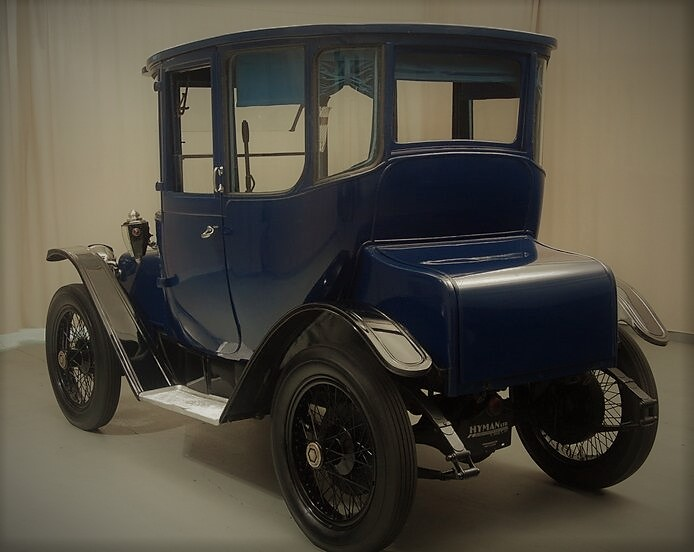
\includegraphics[width=0.75\textwidth]{images/Ende.jpg}
	\label{fig:Ende}
\end{figure}


\color{black}